\chapter{Anforderungsanalyse}\label{chap:requirements}
\fixme{transitions between sections}

\section{Produktüberblick}\label{sec:product_overview}
Zum tiefgreifenderen Verständnis der Anforderungen an das zu entwickelnde Architekturkonzept, muss zunächst einmal der Ausgangszustand, das heißt der jetzige Desktopclient des \nameformat{\gls{crm}} betrachtet werden. Wie am Begriff \gls{CRM} bereits zu erkennen, handelt es sich dabei um ein Programm, das der Verwaltung und Vernetzung von Kunden- und Kontaktdaten dient. Neben den typischen Einsatzbereichen von \gls{CRM}-Produkten, wie die Verwaltung von Kundendaten, Terminen und Aufgaben, legt die combit GmbH allerdings besonderen Wert darauf das Programm möglichst flexibel zu gestalten, um dadurch zahlreiche Kundengruppen mit ihren spezifischen Anforderungen an die Einsatzbereiche der Software zu bedienen. Einige Beispiele hierfür sind die mitgelieferten, fertigen Lösungen (im Kontext des \nameformat{\gls{crm}} \nameformat{Solutions} genannt), mit denen unter anderem Immobilien gehandhabt, die Vermittlung von Arbeitsstellen an Drittfirmen organisiert oder ein Ticket-System aufgebaut werden können. Zudem ist eine Musterlösung für den \gls{dsgvo}-konformen Umgang mit sämtlichen Daten integriert. Unabhängig von diesen Lösungen stehen bestimmte Funktionalitäten durchweg zur Verfügung: Import und Export von Daten in viele verschiedene Formate, Versand von (Serien-) E-Mails oder etwa die Generierung von Berichten (Reports) durch ein zweites internes Produkt ``List \& Label''. Diese bauen jedoch auf den Daten einer Lösung auf.
Eine \nameformat{Solution} stellt die grundsätzliche Organisation der Daten in bestimmte Bereiche oder Szenarien dar und kann von jeder Firma individuell konfiguriert werden. Jede Solution ist durch eine Menge von Datenbanktabellen und darauf basierenden Ansichten zur Visualisierung der in den Tabellen enthaltenen Entitäten und Relationen definiert. In der in Abbildung~\ref{fig:crm_ui} gezeigten Standard-Solution ``Large'' ist links eine Liste der verfügbaren Ansichten und rechts die Detailansicht einer Entität der ``Firmen''-Ansicht zu sehen. Außerdem wird hier auch die allgemeine Trennung zwischen Haupt-UI und ansichtsspezifischer UI ersichtlich. Anstelle der Detailansicht kann auch eine Listenansicht (tabellenförmige Auflistung aller Entitäten), eine Berichtsansicht, eine Webansicht und eine Kombinationsansicht, bei der sowohl die Übersichtsliste als auch die Details sichtbar sind, angezeigt werden.

\begin{figure}
    \centering
    \captionsetup{justification=centering}
    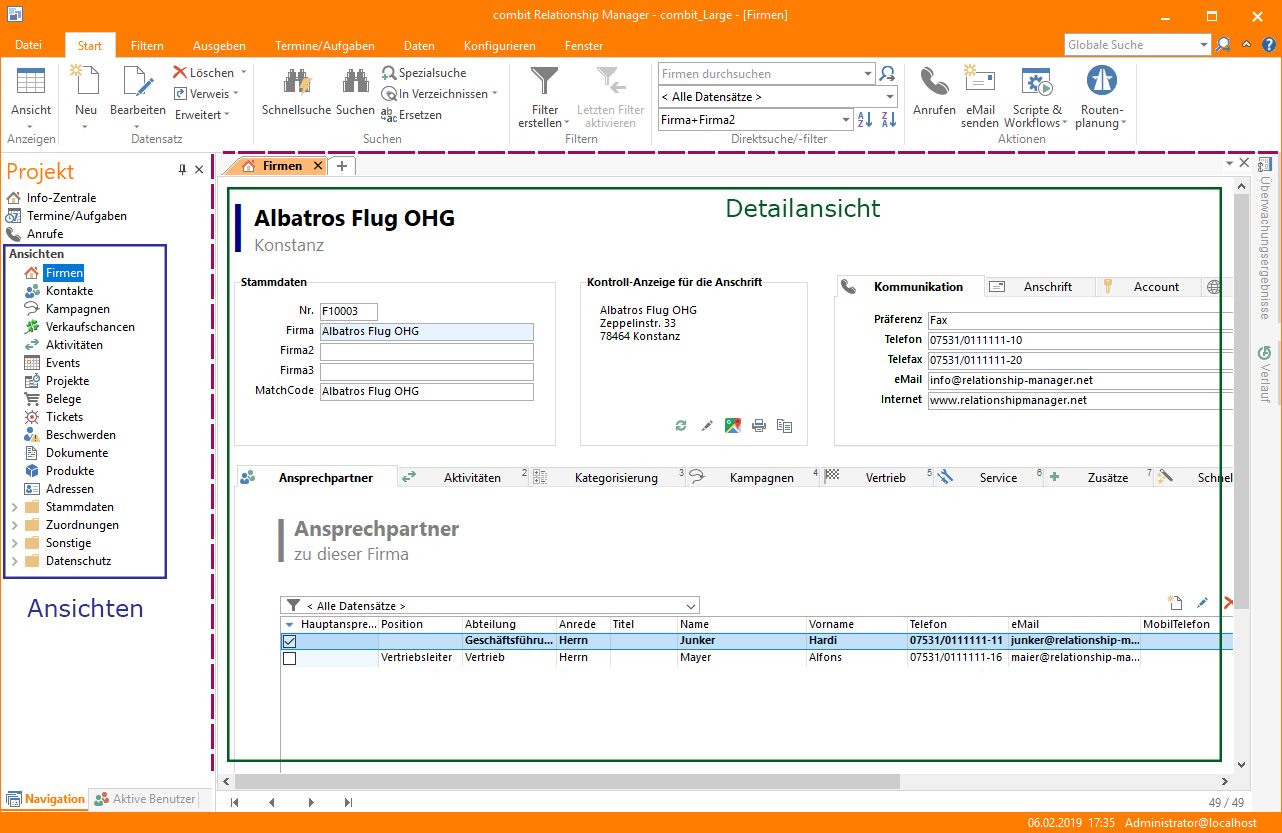
\includegraphics[width=\textwidth]{figures/crm_ui.png}
        \caption{Grafische Oberfläche des \gls{crm} Desktopclient (Februar 2019)}\label{fig:crm_ui}
\end{figure}

Aus technischer Sicht ist der \nameformat{\gls{crm}} in drei Schichten getrennt. Die zu verwaltenden Daten werden entweder in einer Microsoft SQL Server- oder einer PostgreSQL-Datenbank gespeichert. Eine Besonderheit hierbei ist die Tatsache, dass Relationen zwischen Datenbanktabellen nicht durch Fremdschlüssel und zugehörige Relationen auf Datenbankebene, sondern durch virtuelle Relationen zwischen einzelnen Ansichten im C++-Kern der Anwendung, realisiert sind. Dies erlaubt einen flexibleren Umgang mit diesen und vereinfacht das Ändern von Datenbanktabellen, Ansichten und Relationen direkt aus der Oberfläche des \nameformat{\gls{crm}}.
Der \nameformat{\gls{crm}}-Core bildet die zweite Schicht und ist für den Datenbankzugriff und die Business Logic\footnote{Anwendungslogik zwischen UI und Datenbank, welche programmspezifische (Verarbeitungs-) Regeln enthält} verantwortlich. Diese beiden Schichten sollen von der Erstellung der neuen Weboberfläche möglichst unberührt bleiben. Einzig die API-Anbindung für die UI muss an dieser Stelle integriert werden --- betrachtet wird die API in dieser Arbeit jedoch nur aus Sicht der Oberfläche, die Integration im Backend findet zu einem späteren Zeitpunkt statt.
Aufbauend auf dem Kern existieren parallel der Desktopclient, ebenfalls in C++ geschrieben, der WebAccess für Desktopbrowser und der WebAccess Mobile für mobile Endgeräte. Zwischen Core und Webaccess (Mobile) gibt es noch einen mit ASP.NET\footnote{Auf dem .NET-Framework aufbauende Tools und Bibliotheken zum Erstellen von Web-Apps} realisierten .NET-Wrapper, welcher den Zugriff auf Daten per HTTP ermöglicht.

Abbildung~\ref{fig:crm_technical_stack} zeigt eine Übersicht der momentanen Architektur, Abbildung~\ref{fig:crm_future_technical_stack} hingegen, wie die Architektur in Zukunft aufgebaut sein könnte.

\begin{figure}
    \centering
    \captionsetup{justification=centering}
    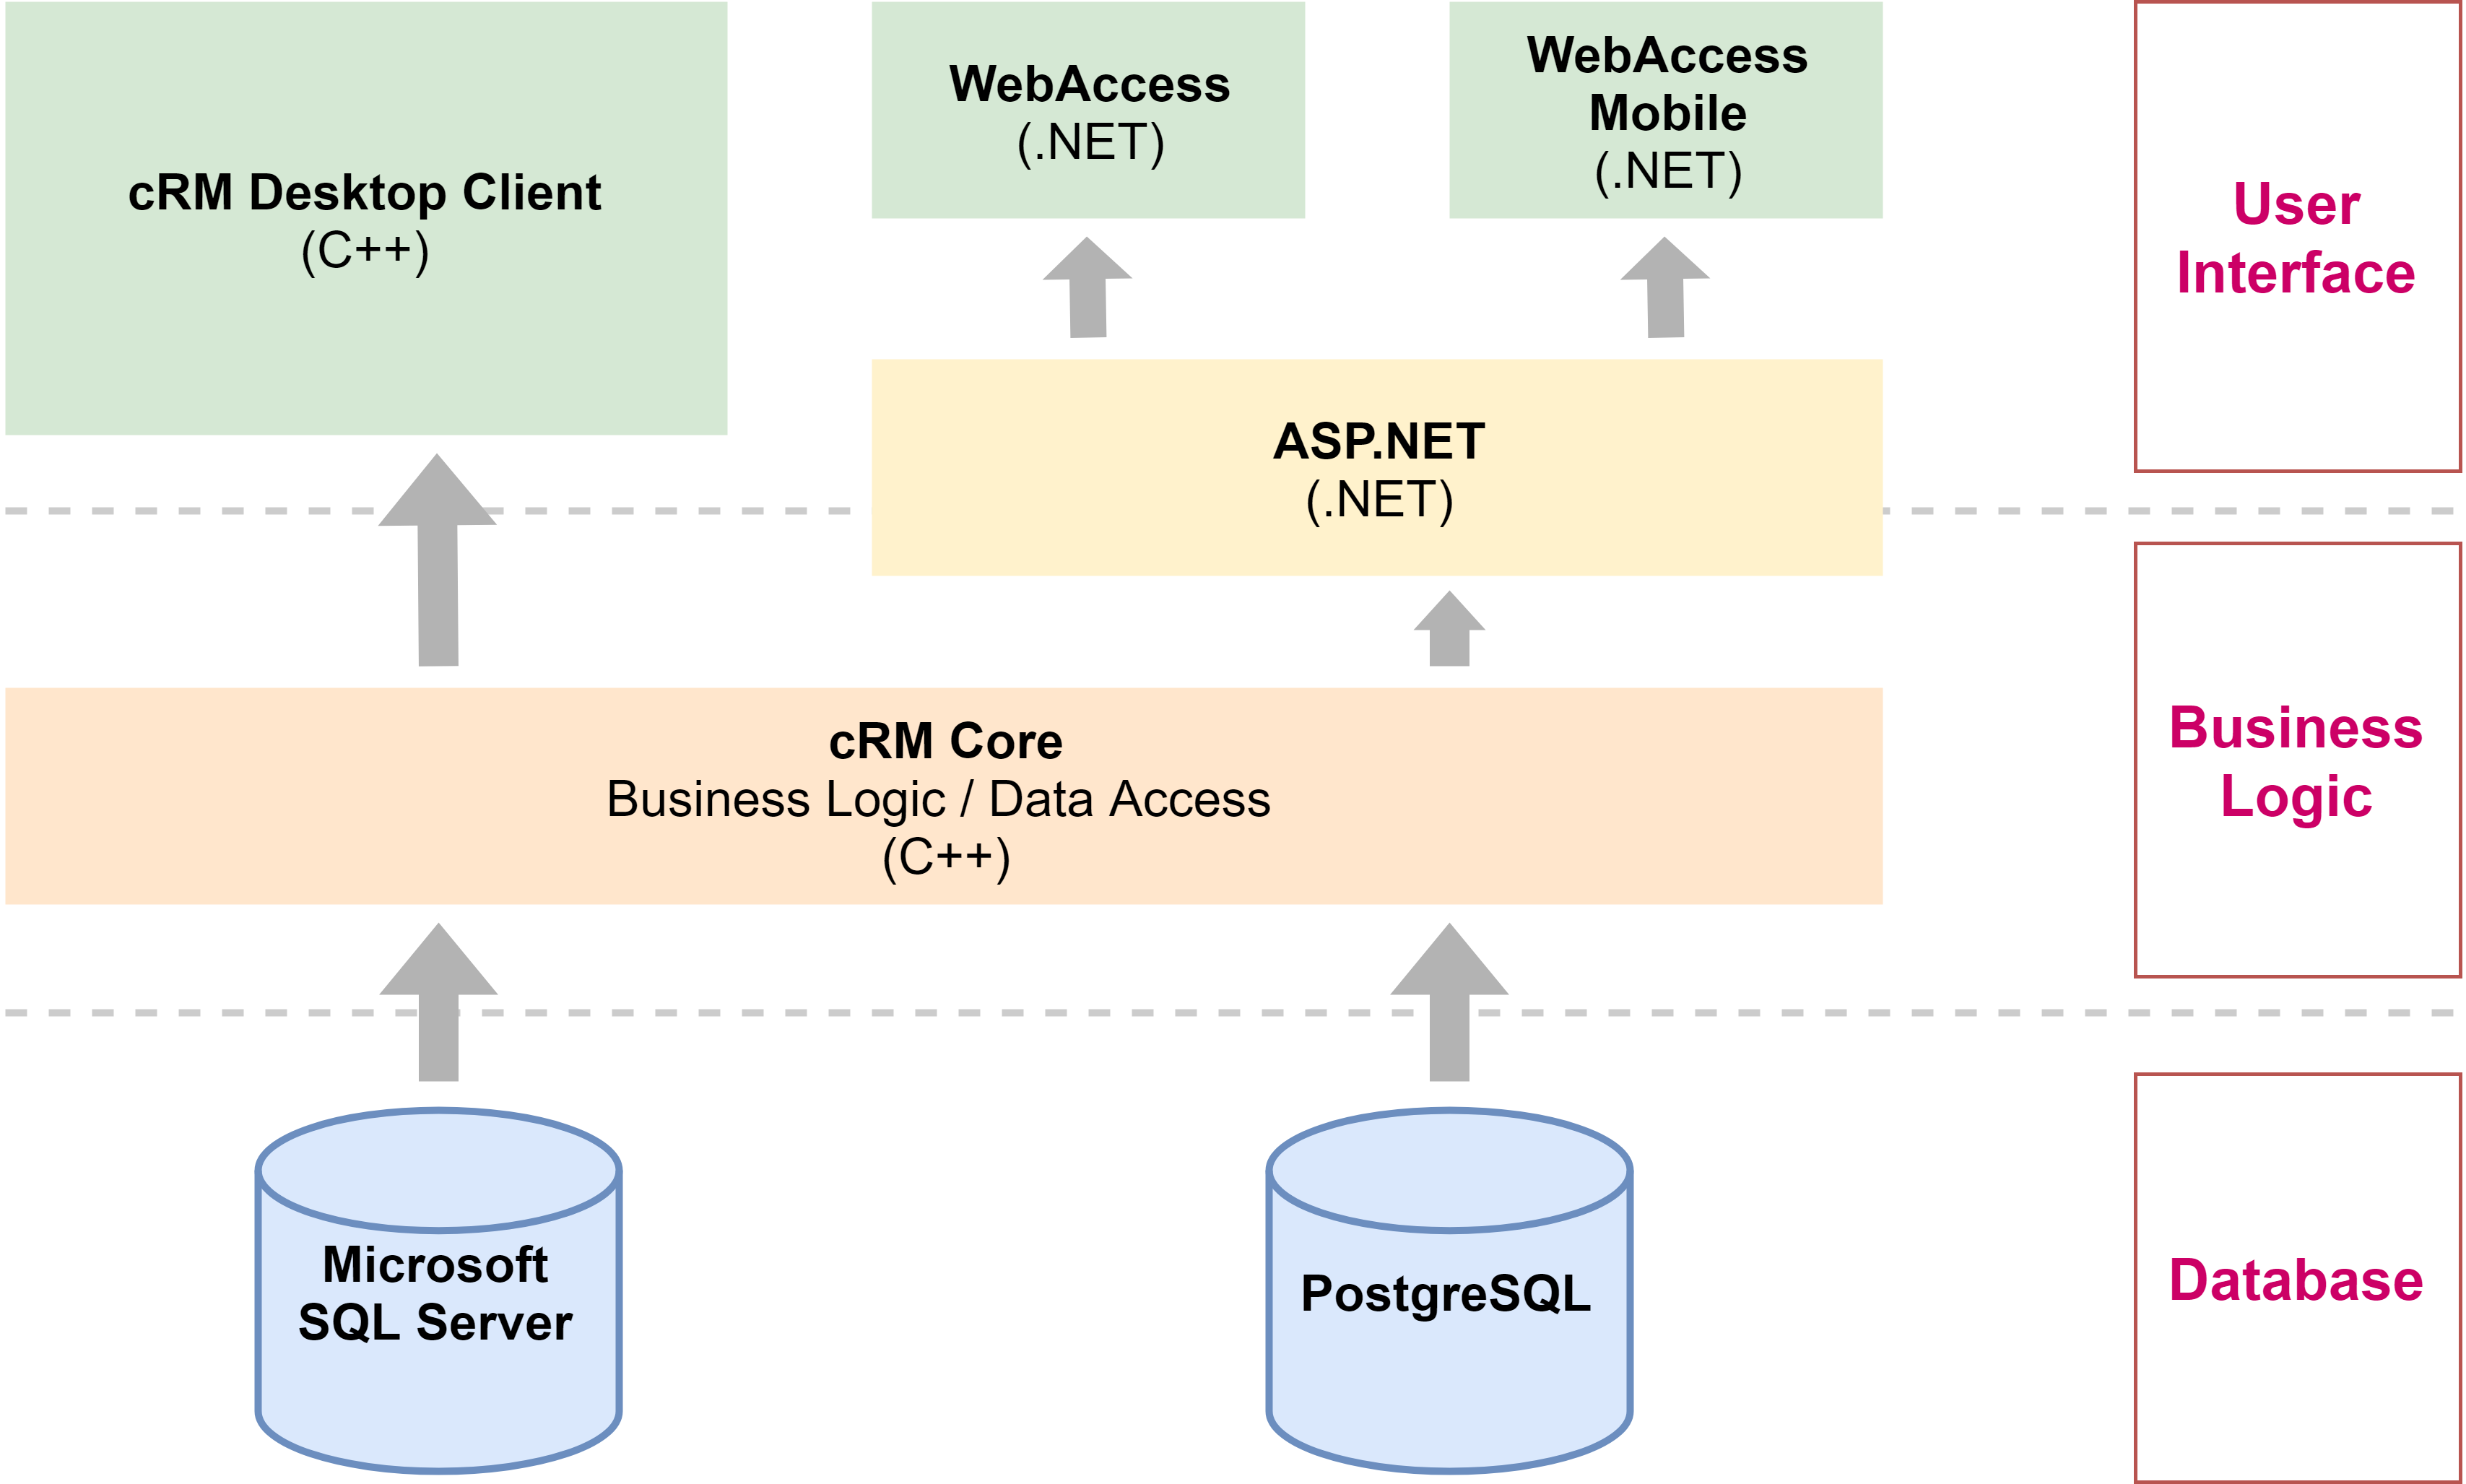
\includegraphics[width=\textwidth]{figures/crm_technical_stack.png}
        \caption{Aktueller technischer Aufbau des \gls{crm}}\label{fig:crm_technical_stack}
\end{figure}

\begin{figure}
    \centering
    \captionsetup{justification=centering}
    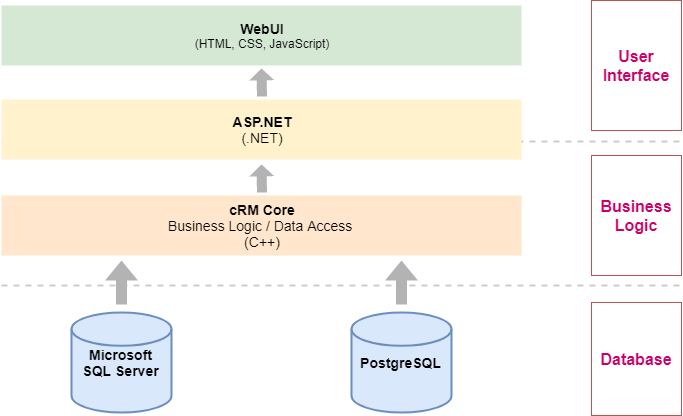
\includegraphics[width=\textwidth]{figures/crm_future_technical_stack.png}
        \caption{Möglicher, zukünftiger technischer Aufbau des \gls{crm}}\label{fig:crm_future_technical_stack}
\end{figure}


\section{Funktionale Anforderungen}
In diesem Teil des Kapitels werden funktionale Anforderungen, welche die Web-UI unterstützen soll, aufgelistet und kurz erläutert. Der erste Abschnitt befasst sich mit Anforderungen, die sich aus dem \gls{crm} ergeben, der zweite Abschnitt mit Anforderungen, die sich aus Web-Apps ergeben.

\subsection{\acrlong{crm}}
\subsubsection{Automatisierte Erstellung}
Die meisten Kunden haben entweder bereits ihre eigenen Ansichten erstellt oder benutzen angepasste Versionen der mitgelieferten Designs. Wird als langfristiges Ziel definiert, die komplette UI-Schicht ins Web zu überführen, muss das Ergebnis dieses Prozesses für die Benutzer leicht und zugänglich genug sein, um nicht schon im Voraus abgelehnt zu werden. Es ist daher essenziell, dass sämtliche bisherigen Ansichten mit minimalem Aufwand seitens der Nutzer im Web weiterverwendet werden können. Der minimale Aufwand meint dabei, dass im Ergebnis lediglich kleine Anpassungen tolerierbar sind, jedoch nicht die Neuerstellung jeder einzelnen Ansicht. Eines der Hauptziele dieser Arbeit ist es daher, eine automatische Umwandlung bestehender Ansichten zu ermöglichen. Hierfür muss die aktuelle UI-Spezifikation analysiert und eine neue Spezifikation erstellt werden, mithilfe derer Implementierungen aus den vorherigen abgeleitet werden können.

\subsubsection{Benutzerverwaltung}
Die Benutzer und deren Rechte werden vollständig im Backend verwaltet. Es muss allerdings bei der Umsetzung der Konfigurationsoberfläche und bei der Umsetzung der Rechte besonders sorgfältig geprüft werden, ob weiterhin der volle Funktionsumfang gewährleistet ist. Sollten bestimmte Rechte für Benutzer oder Gruppen nicht mehr anpassbar sein  oder fehlerhaft angewendet werden, ist unter Umständen der gesamte \nameformat{\gls{crm}} nicht mehr vernünftig nutzbar.

\subsubsection{Edit-Modus}
Änderungen in der Detailansicht werden nicht direkt an die Datenbank übertragen, sondern nur als geändert markiert. Der Benutzer hat dann die Möglichkeit diese zu verwerfen oder den entsprechenden Datensatz zu speichern und die Informationen in die Datenbank zu schreiben.

\subsubsection{Individualisierung}
Die Individualisierung der beiden Hauptansichten für Datenentitäten, die Detail- und Listenansicht, ist zur effektiven Visualisierung bestimmter Sachverhalte ausschlaggebend. Bei der Listenansicht können beispielsweise Datenbankspalten ein- bzw.\ ausgeblendet und frei angeordnet werden, Spalten je nach Datentyp formatiert und spezielle Werte nach selbst definierten Regeln hervorgehoben werden. Die Detailansicht ist noch mächtiger, hier kann jedes UI-Element frei platziert werden, mit Sichtbarkeits- und Formatierungsbedingungen versehen und mit anderen Feldern verknüpft werden (verknüpft bedeutet: Änderung in Feld A löst Änderung in Feld B aus). Um diese Einstellungen vorzunehmen, ist ein Eingabemaskendesigner in die Software integriert, welcher dem Benutzer per ``\gls{wysiwyg}''-Prinzip\footnote{Echtzeitdarstellung des Ergebnisses während der Erstellung und Bearbeitung} das Designen erleichtert.
Die Weboberfläche sollte diese Funktionalität möglichst vollständig abbilden.

\subsubsection{Berichts- und Webansicht}
Wie in Abschnitt~\ref{sec:product_overview} erwähnt, werden Berichte von einem zweiten Produkt der Firma \nameformat{combit GmbH}, dem sogenannten \nameformat{\gls{ll}}, gehandhabt. Dieses besitzt bereits zum jetzigen Zeitpunkt eine entsprechende Weboberfläche, die zukünftig für die Erstellung und das Anzeigen von Berichten genutzt werden kann. 
Auch die Webansicht kann weiterhin unterstützt werden, indem darin anzuzeigende Ressourcen in ein iframe-Tag\footnote{HTML-Element, welches das Einbetten von Dokumenten in andere Dokumente erlaubt} eingebunden werden.

\subsubsection{Suche / Filter / Sortierung}
Das Suchen und Filtern von Datensätzen kann weiterhin mit bestehenden Techniken gelöst werden, indem das Backend Daten vor dem Senden entsprechend im Vorfeld verarbeitet. Da es allerdings sinnvoll ist, Sortierungen in der Übersichtsliste auf dem Client auszuführen --- eine Garantie der API, dass Daten immer in einer entsprechenden Reihenfolge gesendet und auch empfangen werden, schränkt das Design dieser zu sehr ein --- ist es zumindest überlegenswert, ob das Suchen und Filtern ebenfalls zusätzlich direkt auf dem Client unterstützt werden soll. Viele JavaScript-Projekte bieten hierfür bereits fertige und effiziente Lösungen an, welche bei der Umsetzung genutzt werden können.

\subsubsection{Scripting}
Die Desktopanwendung des \nameformat{\gls{crm}} unterstützt momentan das Ausführen von Skripten in den Sprachen VBScript und C\#. Für die programmatische Ansteuerung existiert eine \gls{COM}-API, welche im Kontext des Clients, auf dem der Prozess ausgeführt wird, benutzt werden kann. Diese Technologien sind in einer Browserumgebung nicht verfügbar, daher kann ein Skript zwar über die neue UI ausgelöst, aber nicht lokal, sondern ausschließlich im Kontext des Servers ausgeführt werden. Existierende Skripte, welche darauf ausgelegt sind im Kontext des Clients ausgeführt zu werden, müssen vor der Nutzung in der Web-UI entsprechend angepasst werden.

\subsubsection{Import / Export}
Der Import und Export von Daten in und aus dem \nameformat{\gls{crm}} ist ein wichtiges Feature, wenn es darum geht, verschiedene Programme in einem Workflow zu vereinen. Der \nameformat{\gls{crm}} unterstützt diese Funktion mit einer Vielzahl an Formaten (Excel, Outlook, Datenbanken (ODBC) und Weitere). Diese Funktion kann, wie viele andere auch, weiterhin bestehen bleiben. Dafür muss jedoch eine Möglichkeit geschaffen werden, die Daten über das Netzwerk zur Verfügung zu stellen (Down- und Upload).

\subsubsection{Terminverwaltung und Aufgabenplanung}
Die interne Termin- und Aufgabenverwaltung ist analog zu anderen Daten über Datenbanktabellen realisiert. Diese können ebenso vom Backend an die Web-UI übertragen und dort dargestellt werden. Der Desktopclient unterstützt aber zudem auch die Verwaltung von Terminen von externen Programmen (z.B. \nameformat{Microsoft Outlook}). Eine Anbindung der neuen UI an diese kann nur gewährleistet werden, wenn entsprechende HTTP-APIs von den Produkten angeboten werden.

\subsubsection{Design für mobile und stationäre Endgeräte}
Da die neue Oberfläche alle bisherigen UI-Versionen ablösen soll, ist es ein zentrales Anliegen, sämtliche Endgeräte ihrer Möglichkeiten nach zu unterstützen. Eine bewährte Herangehensweise besteht darin, das mobile Design vor der Desktop-Ansicht zu gestalten. So können die wichtigsten Eigenschaften und Fähigkeiten des Designs direkt angelegt werden, während das Design für größere Bildschirme darauf aufbauend mit zusätzlichen Features, die speziell hierfür sinnvoll sind, ergänzt werden. Dieses Prinzip wird häufig ``mobile-first''-Design genannt. Bei einer umgekehrten Vorgehensweise wird zuerst die Desktop-Ansicht mit allen verfügbaren Features und unter Ausnutzung des gesamten Bildschirmplatzes gestaltet. Dieses Design muss dann für mobile Geräte kompatibel gemacht werden, indem Features und Designelemente entfernt werden. Die Entscheidung, welche Aspekte dabei entfernt werden können, ist schwierig, da sie alle essenziell erscheinen.
Es ist zusätzlich auch wichtig zu beachten, dass viele mobile Nutzer --- je nach Standort --- keine ausreichend gute oder zumindest nur eine teilweise gute Internetverbindung besitzen und es daher wichtig ist, möglichst wenig Daten übertragen zu müssen, bevor eine Webseite angezeigt wird. Das für mobile Geräte charakteristische CSS sollte zuerst geladen werde, da dies weitere Downloads von irrelevanten Daten (CSS für nicht-mobile Geräte) vermeidet. Für stationäre Geräte ist eine derartige Optimierung jedoch nicht vonnöten.

\subsubsection{Vorerst nicht unterstützte Features}
Einige aktuelle Features des \gls{crm}s sind im Web entweder gar nicht oder nur mit sehr viel Aufwand umsetzbar. Diese werden daher vorerst nicht weiter beachtet und deren Umsetzbarkeit eventuell zu einem späteren Zeitpunkt erneut betrachtet:

\fixme{itemize alternative?}
\begin{itemize}
    \item{Scripting-Unterstützung auf dem Client}
    \item[] Skripte werden momentan immer auf dem Client ausgeführt und evaluiert, dabei existiert u.a. Zugriff auf das Dateisystem und andere native Anbindungen des Betriebssystems. Da eine Webseite in der Browserumgebung aus Sicherheitsgründen vom restlichen Betriebssystem isoliert ist, können diese Möglichkeiten nicht genutzt und eine direkte Skriptausführung daher nicht unterstützt werden. 
    \item{Interaktion mit anderen Prozessen}
    \item[] Bisher war es möglich, mit anderen Prozessen auf dem Client zu interagieren (Starten von externen Programmen, Interkation mit diesen per \gls{COM}, etc.). Ein Beispiel hierfür ist ein Hilfsprogramm, mit dem Anrufe direkt am PC entgegengenommen und automatisch im \nameformat{\gls{crm}} protokolliert werden können. Eine derartige Interaktion ist in einer Browserumgebung, vor allem in einem, von fast allen gängigen Browsern benutzten Sandbox-Modus, nicht möglich.
    \item{Ereignisse} 
    \item[] Ereignisse sind Events, die zu bestimmten Zeitpunkten der Programmlaufzeit ausgelöst werden und als Aktion zum Beispiel ein Skript starten oder eine E-Mail versenden können. Bevor diese in der Web-UI implementiert werden können, muss zuerst evaluiert werden, welche dieser Ereignisse noch unterstützt werden können (Beispiel: Das Event ``Nach Programmstart'' --- anstatt eines Prozesses existiert nur noch eine Webseite. Das Laden dieser ist nicht gleichbedeutend mit dem Starten eines Prozesses, daher kann dieses Ereignis nicht mehr unterstützt werden.)
\end{itemize}

\subsection{Webbereich}
Zusätzlich zu diesen Anforderungen gibt es im Web noch diejenigen Bereiche, die unterstützt werden sollten, um den Nutzern eine besonders gute Erfahrung bei der Bedienung der Seite zu ermöglichen, und solche Bereiche, die den Entwicklungsprozess positiv beeinflussen. Die wichtigstem dieser Anforderungen werden im Folgenden kurz erläutert. 

\subsubsection{i18n / i10n}
Die Akronyme ``i18n'' und ``i10n'' stehen für Internationalisierung respektive Lokalisierung \parencite{i18n_i10n_ishida_w3c_miller_boeing_2018}. Gemeint ist damit, dass für jede Sprachressource auf einer Webseite anstelle des Strings ein Identifikator genutzt wird, der mit Strings verschiedener Sprachen verknüpft ist. Je nach Einstellung (Auswahl durch Benutzer, Erkennung der Browsersprache, etc.) können dann automatisch alle Texte in der jeweiligen Sprache angezeigt werden. Der \nameformat{\gls{crm}} unterstützt bereits mehrere Sprachen, die Ressourcen hierfür sind allerdings direkt in das Programm eingebettet. Um die gleiche Technologie für die Webseite nutzen zu können, müssten also sämtliche Texte durchweg aus dem Backend angefordert und über das Internet übertragen werden. Dies wäre nicht nur langsam und eine unnötige Belastung für den Server (Texte müssten bei jedem Aktualisieren der UI-Schicht neu geladen werden), sondern auch sehr fehleranfällig. Bei einer unterbrochenen Verbindung könnten überdies keine Fehlertexte angezeigt werden. Besonders im Hinblick auf den weiter unten beschriebenen ``offline-first''-Ansatz sollten daher sämtliche Texte in der UI-Schicht gespeichert und jederzeit abrufbar sein.

\subsubsection{Barrierefreiheit}
Barrierefreiheit von Software bedeutet, dass diese auch von Menschen mit körperlichen Einschränkungen gut genutzt werden kann. Dies ist selbstverständlich immer ein wünschenswertes Ziel, zahlreiche Standards im Webbereich erleichtern ein solches Vorhaben jedoch in besonderem Maße. So gibt es beispielsweise bestimmte HTML-Tags, die extra dafür geschaffen wurden, um von Sprachsoftware vorgelesen zu werden. Weiterhin besteht die Möglichkeit per austauschbarem CSS einen ``Dark Mode'' anzubieten, sofern ein System von Beginn an entsprechend aufgebaut wurde.
Es sollte daher herausgearbeitet werden, welche Möglichkeiten für eine hohe Barrierefreiheit existieren und wie diese bei der Softwareentwicklung beachtet und umgesetzt werden können.

\subsubsection{Anleitungs-Modus / ``Feature-Tour''}
 Um neuen Nutzern den Einstieg beim Erlernen eines Produkts zu erleichtern, kann ein interaktiver Anleitungs-Modus, welcher entweder beim ersten Aufruf einer Webseite und~/~oder bei der ersten Nutzung einzelner Features ausgelöst wird, hilfreich sein. Ein solcher Modus hebt wichtige Bedienelemente hervor und gibt kurze Erklärungen zu ebendiesen, welche entweder direkt durch einen Klick beendet werden können oder intelligent seltener erscheinen, je länger der jeweilige Nutzer das Produkt bereits kennt. Eine mögliche, fertige Umsetzung eines solchen Modus ist in Abbildung~\ref{fig:intro_js_example} von \nameformat{Intro.js} dargestellt.

 \begin{figure}
    \centering
    \captionsetup{justification=centering}
    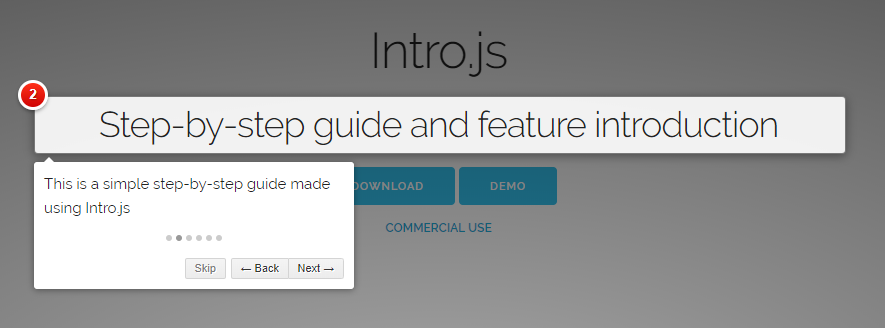
\includegraphics[width=\textwidth]{figures/intro_js_example.png}
        \caption{Anleitungs-Modus von Intro.js \parencite{mehrabani}}\label{fig:intro_js_example}
\end{figure}

\subsubsection{``Offline-First''-Ansatz}
In jüngster Zeit ist es möglich, mithilfe von Service-Workern\footnote{JavaScript-Proxy zwischen Webseite und Server; wird in einem anderen Thread als die eigentliche Webseite ausgeführt und kann Anfragen abfangen / verändern} und lokalen Speichermöglichkeiten im Browser Webseiten zu erstellen, die auch beim Aussetzen der Internetverbindung zumindest im Wesentlichen weiterhin funktionieren. So können etwa Änderungen, welche an den Server geschickt werden müssen, zwischengespeichert und, sobald wieder eine Verbindung zum Internet besteht, losgeschickt werden. Ein weiteres Beispiel ist das Anzeigen von Daten, die vom letzten Besuch einer Seite stammen, wenn beim aktuellen Aufruf die Verbindung nicht stabil genug ist. Natürlich sollte ein Nutzer über Änderungen des Status der Internetverbindung informiert werden.
Die Information über Verbindungsprobleme sowie die Antizipation ebendieser durch lokales Speichern von relevanten Informationen, zielen beide auf eine für mobile Nutzer möglichst komfortable Bedienung einer Webseite ab, was wie zuvor erwähnt, ein Hauptaugenmerk der neuen Oberfläche darstellt.

\subsubsection{Intelligente Fehlerbehandlung}
Softwarefehler auf eine für den Benutzer angenehme Art und Weise zu behandeln und im Nachhinein detailliert zu analysieren, ist bei traditioneller Software ein nicht zu unterschätzendes Problem. Bei Webapplikationen kommt jedoch erschwerend hinzu, dass ein Teil der Logik in einer Umgebung ausgeführt wird, welche durch herkömmliche Mittel nicht untersucht werden kann (Browser auf Clientrechner). Umso wichtiger ist es, ein Konzept zu entwickeln, welches in der entsprechenden Umgebung auftretende Fehler sowie Informationen zu deren Lösung übermittelt. Eine Option zur Lösung des Problems bestünde darin, auftretende Fehler immer direkt zum Server zu schicken, um sie vor Ort analysieren zu können. Wenn die eigene Infrastruktur dafür nicht ausreichend ausgebaut ist, gibt es auch entsprechende Online-Dienste, welche die Speicherung eines solchen Fehlerlogs ermöglichen. Zusätzlich dazu müssen auch Parameter für Serveranfragen mit höchster Vorsicht ausgewählt werden: Timeouts müssen lange genug sein, um eine Serverantwort nicht fälschlicherweise zu verwerfen und kurz genug, um bei einem tatsächlichen Fehler die Applikation nicht zu träge wirken zu lassen. Zudem sollten im Fehlerfall erneute Versuche intelligent gestartet werden, das heißt weder zu häufig noch zu selten, um den Server nicht unnötig zu belasten respektive um dennoch einen responsiven Eindruck zu vermitteln.

\subsubsection{Etablierte Authentifizierung}
Der \nameformat{\gls{crm}} besitzt zwar bereits ein integriertes Benutzersystem mit Rechteverwaltung, für die Portierung der Oberfläche sollte aber in Erwägung gezogen werden, diese Rechteverwaltung mit einem oft genutzten, öffentlichen Protokoll wie \nameformat{OAuth} oder ähnlichen Protokollen zu koppeln, um die Verbindung über HTTP und den Schutz der Authentisierungsdaten nicht mit einer selbst entwickelten, schlechter funktionierenden Lösung handhaben zu müssen.

\subsubsection{Caching}
Um Ressourcen zu sparen, ist es von Vorteil komplexe Berechnungen und zeitintensive Übertragungen nicht mehrmals, etwa bei mehrfachem Laden einer Webseite, auszuführen. Im Bereich des Webs gibt es mehrere Möglichkeiten solche Daten temporär zu speichern: Die einfachste Form besteht darin, Antworten auf eingehende Anfragen auf dem Server und ebenso danach auf dem Client wiederzuverwenden. Wenn der Client selbst kein Caching unterstützt, kann mit ``bedingten Anfragen'' dennoch der Cache des Servers genutzt werden: Es wird hierbei eine Anfrage an den Server geschickt und, sollte sich die Antwort im Vergleich zur letzten Anfrage nicht geändert haben, keine Daten, sondern nur ein entsprechender Hinweis an den Client zurückgesendet. Auch das HTTP-Protokoll unterstützt Mechanismen um Caching, beispielsweise über Cache-Proxies, zu erleichtern (spezielle Header, welche die Gültigkeitsdauer einer gespeicherten Ressource bestimmen). Bei allen Formen des Caching ist es jedoch kritisch, dass die richtige Strategie zum Invalidieren der Daten ausgewählt wird, um nicht mit veralteten Werten zu arbeiten, aber dennoch eine Effizienzsteigerung zu erreichen.

\subsubsection{Container}
Container-Technologien wie Docker und Kubernetes helfen dabei Abhängigkeiten der eigenen Software zu verwalten und auf jedem Entwicklungsrechner eine identische Umgebung zu schaffen. Auch für die Bereitstellung eines Service für Kunden ist es sehr viel einfacher einen bereits korrekt konfigurierten Container zu starten, anstatt eine vollständige Umgebung auf einem Server einzurichten. Dies gilt insbesondere wenn dieser Server von externen Dienstleistern verwaltet wird. Da diese Konzepte bei der \nameformat{combit GmbH} noch nicht eingesetzt werden, ist es sinnvoll zu untersuchen, an welchen Stellen diese zu mehr Produktivität in Entwicklung und Verteilung der Software beitragen könnten.

\subsubsection{Serverless}
Unter ``Serverless'' wird das Konzept verstanden, dass Firmen keine eigenen Server für ihre Kunden oder eigene Zwecke einrichten müssen, sondern auf Lösungen von Drittherstellern (etwa \nameformat{AWS} von \nameformat{Amazon} oder \nameformat{Microsoft Azure}) zurückgreifen können, auf welchen die eigene Software ausgeführt wird. Firmenintern wird also kein Server betrieben, die eigene Infrastruktur ist demnach ``Serverless''. Der Vorteil dieses Ansatzes ist, dass die Verantwortung über die Serverhardware nicht selbst getragen werden muss und die Server durch die großen Kapazitäten der Hersteller je nach Belastung skaliert werden können. Im Gegenzug werden aber eigene Daten fremden Servern anvertraut, je nach Art und Sensibilität der Daten (Betriebsgeheimnisse, \gls{dsgvo}) kann dies nicht gewünscht sein. Ein solcher Ansatz muss daher gut abgewogen werden, bevor er weiter verfolgt werden kann.

\subsubsection{Aktualisierungsstrategie}
Kontinuierliche Softwareupdates zur Fehlerverbesserung oder zur Ergänzung neuer Features zählen heutzutage zum Standardservice. Wenn dieser Service angeboten werden soll bedarf es einer kompetenten Strategie, um Modifikationen und Erweiterungen an die Nutzer auszuliefern. Das Backend, auf dem auch die UI-Schicht gehostet werden soll, wird von den Kunden betrieben. Es unterliegt damit nicht dem Verwaltungsbereich der \nameformat{combit GmbH}, weshalb Updates nicht direkt dort eingespielt werden können. Anstatt Updates für die Oberfläche an Updates des Backends zu koppeln, sollte überlegt werden, ob eine konfigurierbare Option angeboten werden kann, durch die Updateprüfungen auf einem zentralen \nameformat{combit}-Server ausgeführt werden. Dies setzt allerdings voraus, dass verschiedene Versionen der Oberfläche und des Backend miteinander kompatibel sind. 

\subsubsection{Integration von bestehenden Ressourcen}
Auf der Webseite der \nameformat{combit GmbH} gibt es bereits zahlreiche Ressourcen wie FAQ oder eine Knowledgebase zu verschiedenen Produkten. Um Nutzern diese Ressourcen präsent zu machen, könnten diese direkt in die Oberfläche, etwa im Rahmen eines Hilfe-Modus, integriert werden.

\section{Anforderungen an den Entwicklungsprozess}
Neben den funktionalen Anforderungen ist es ebenso wichtig, die richtigen Anforderungen für die Projektumgebung und -entwicklung zu formulieren, um diesen Prozess möglichst effizient und skalierbar zu halten. Daher wird empfohlen, folgende Technologien und Praktiken bei der Entwicklung des neuen Projektes zu nutzen:

\fixme{itemize alternative?}
\begin{itemize}
    \item{Tests}
    \item[] Alle in Kapitel~\ref{chap:technologies} vorgestellten UI-Frameworks enthalten bereits Lösungen zur Ausführung von Tests. Eine hohe Testabdeckung ist daher nicht nur nützlich, um die Codequalität zu erhalten und Regressionen zu erkennen, sondern auch ohne hohe Kosten und Aufwand erreichbar.
    \item{Continuous Integration}
    \item[] Ein für diesen Zweck geeigneter \nameformat{TeamCity}-Server von der Firma \nameformat{JetBrains} ist firmenintern bereits vorhanden, daher sollten Tests von neuen Features immer auch auf diesem Server ausgeführt werden.
    \item{Codereviews}
    \item[] Pro Feature sollte auf einem gesonderten Branch gearbeitet und beim Zurückführen in den Masterbranch ein Review durch mindestens einen anderen Entwickler stattfinden, um die Codequalität stets auf einem hohen Niveau zu halten. Auch für Reviews gibt es firmenintern bereits einen \nameformat{Upsource}-Server (ebenfalls von der Firma \nameformat{JetBrains}), welcher mit dem \nameformat{TeamCity}-Server zusammen genutzt werden kann.
\end{itemize}

\section{Hauptaugenmerk dieser Arbeit}
Eine komplette Umsetzung aller Anforderungen wäre im Rahmen dieser Thesis nicht zu bewältigen. Es gäbe zu viele Aspekte (geeignetes Hosting, eine sichere Authentifizierungsmethode, ein neuer Aktualisierungsmechanismus, etc.), die beachtet werden müssen. Summiert reicht die Zeit nicht aus, um Konzepte für all diese Aspekte in einer entsprechenden Qualität und Sorgfalt zu erstellen und umzusetzen. 
Wie in diesem Kapitel bereits beschrieben, kann die Oberfläche des \nameformat{\gls{crm}} in zwei Hauptbereiche unterteilt werden. Zum einen existieren diejenigen UI-Bereiche, welche sich nicht mit den anzuzeigenden Daten ändern, wie in Abbildung~\ref{fig:crm_ui} links und oberhalb der Detailansicht erkennbar wird (weitere Dialoge und Oberflächen werden kontextbasiert angezeigt), und zum anderen die Detail- und Listenansicht selbst. Die nicht datenabhängigen Elemente und Dialoge bestehen fast vollständig aus statischen Elementen mit teilweise speziellen Anforderungen, welche bei der Umsetzung zwar zeitaufwändig wären, technisch jedoch kein interessantes Problem darstellten. Es werden im Weiteren daher nur die Oberfläche der Datenansichten (Detail- und Listenansicht) und die damit verbundenen Anforderungen betrachtet. 

Aus der Liste der funktionalen Anforderungen des \nameformat{\gls{crm}} werden also insbesondere folgende Punkte beachtet:
\begin{itemize}
    \item{Automatisierte Erstellung}
    \item{Editier-Modus}
    \item{Individualisierung}
    \item{Suche / Filter / Sortierung}
\end{itemize}

Ein Vorteil von moderner, komponentenbasierter Webtechnologie (alle in Kapitel~\ref{chap:technologies} betrachteten Frameworks sind darauf ausgelegt) ist es, trotz der getrennten Entwicklung verschiedener UI-Bestandteile diese problemlos miteinander zu kombinieren zu können. Es ist sogar möglich unterschiedliche Technologien für die jeweiligen Teile zu nutzen, da zur Laufzeit alle Framework-Umsetzungen in herkömmliches JavaScript, HTML und CSS transpiliert\footnote{Übersetzung von Quellcode aus einer Programmiersprache in eine andere} werden und somit miteinander kompatibel sind.
Bei dieser zweistufigen Umsetzung kann das Ergebnis dieser Arbeit außerdem bereits in der Webansicht der bestehenden Desktopapplikation angezeigt und als Alternative zu den nativen Oberflächen angeboten werden. So können Kunden dieses Feature bei Interesse bereits im Vorfeld testen, evaluieren und wichtiges Feedback für die weitere Entwicklung einbringen.
